\documentclass[aspectratio=169]{beamer}
\usetheme{Boadilla}
\usecolortheme{default}
\definecolor{primary}{RGB}{43, 87, 154}
\definecolor{accent}{RGB}{221, 75, 57}
\definecolor{good}{RGB}{46, 139, 87}
\setbeamercolor{structure}{fg=primary}
\setbeamercolor{title}{fg=primary}
\setbeamercolor{frametitle}{bg=primary, fg=white}
\setbeamertemplate{navigation symbols}{}

\usepackage{tikz}
\usetikzlibrary{shapes.geometric, arrows.meta, positioning, fit, calc, decorations.pathreplacing}
\usepackage{graphicx}
\usepackage{booktabs}
\usepackage{amsmath}
\usepackage{pgfplots}
\pgfplotsset{compat=1.16}

% ---------- reusable icons ----------
% small graph icon: a hub with 4 neighbours
\hyphenpenalty=10000 \exhyphenpenalty=10000
\newcommand{\icongraph}[1]{%
\begin{tikzpicture}[baseline=-0.5ex,scale=0.35]
  \foreach \a in {45,135,225,315}{\draw[#1,thick] (0,0)--(\a:1);\fill[#1] (\a:1) circle (0.2);}
  \fill[#1] (0,0) circle (0.3);
\end{tikzpicture}}
% cross / check icons
\newcommand{\iconx}{\tikz[baseline=-0.5ex]{\fill[accent] (0,0) circle (0.22cm);\draw[white,line width=1.2pt] (-0.09,-0.09)--(0.09,0.09) (-0.09,0.09)--(0.09,-0.09);}}
\newcommand{\iconok}{\tikz[baseline=-0.5ex]{\fill[good] (0,0) circle (0.22cm);\draw[white,line width=1.2pt] (-0.1,0)--(-0.03,-0.08)--(0.1,0.09);}}

\title[Stress-Testing AnomalyGFM]{Beyond the Baseline: Stress-Testing AnomalyGFM}
\subtitle{A Scientific Autopsy of Graph Foundation Models in Transfer Learning}
\author{Group 13}
\date{November 12, 2026}

\begin{document}

\begin{frame}
    \titlepage
\end{frame}

% --- SLIDE 1 ---
\begin{frame}{The Promise of AnomalyGFM}
    \textbf{The Goal:} Train a Graph Foundation Model once, detect anomalies zero-shot anywhere.

    \begin{center}
    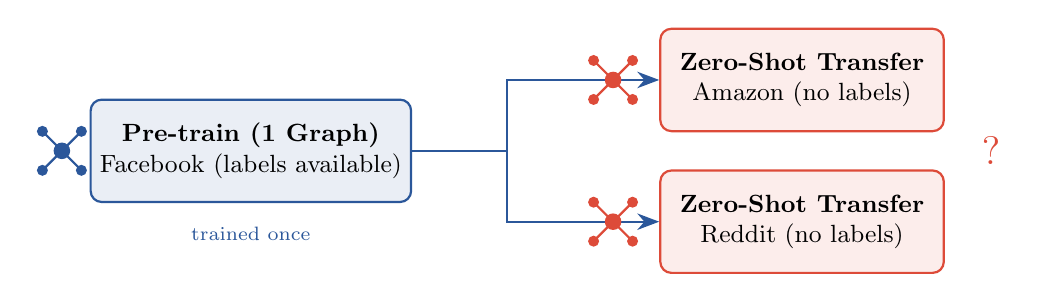
\begin{tikzpicture}[auto, thick,
        box/.style={rectangle, draw=primary, fill=primary!10, rounded corners, minimum width=3.6cm, minimum height=1.3cm, align=center, font=\small},
        arrow/.style={-{Stealth[scale=1.2]}, thick, primary}]

        \node[box] (train) at (0,0) {\textbf{Pre-train (1 Graph)}\\Facebook (labels available)};
        \node[box, fill=accent!10, draw=accent] (test1) at (7,0.9) {\textbf{Zero-Shot Transfer}\\Amazon (no labels)};
        \node[box, fill=accent!10, draw=accent] (test2) at (7,-0.9) {\textbf{Zero-Shot Transfer}\\Reddit (no labels)};
        \draw[arrow] (train.east) -- ++(1.2,0) |- (test1.west);
        \draw[arrow] (train.east) -- ++(1.2,0) |- (test2.west);

        % icons
        \node at (-2.4,0) {\icongraph{primary}};
        \node at (4.6,0.9) {\icongraph{accent}};
        \node at (4.6,-0.9) {\icongraph{accent}};
        \node[font=\scriptsize, primary] at (0,-1.05) {trained once};
        \node[font=\scriptsize, accent] at (9.4,0) {\Large ?};
    \end{tikzpicture}
    \end{center}

    \textbf{The Reality:} Generic models fail here because anomalies are rare, irregular, and highly heterogeneous across domains.
\end{frame}

% --- SLIDE 2 ---
\begin{frame}{Under the Hood: How it Actually Works}
    \textbf{Core assumption:} Normal nodes look like their 1-hop neighbors. Anomalies do not.

    \begin{center}
    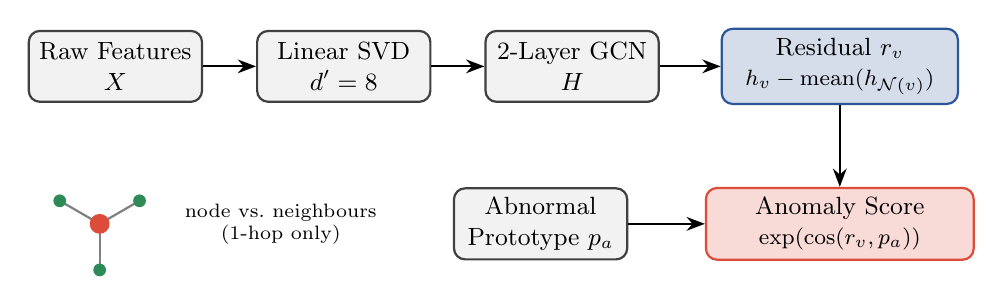
\begin{tikzpicture}[auto, thick,
        stp/.style={rectangle, draw=darkgray, fill=gray!10, rounded corners, minimum width=2.2cm, minimum height=0.9cm, align=center, font=\small},
        arrow/.style={-{Stealth}, thick}]

        \node[stp] (feat) at (0,0) {Raw Features\\$X$};
        \node[stp] (svd) at (2.9,0) {Linear SVD\\$d'=8$};
        \node[stp] (gcn) at (5.8,0) {2-Layer GCN\\$H$};
        \node[stp, fill=primary!20, draw=primary, minimum width=3cm] (res) at (9.2,0) {Residual $r_v$\\{\footnotesize $h_v-\mathrm{mean}(h_{\mathcal N(v)})$}};
        \node[stp, fill=accent!20, draw=accent, minimum width=3.4cm] (score) at (9.2,-2) {Anomaly Score\\{\footnotesize $\exp(\cos(r_v,p_{a}))$}};
        \node[stp] (proto) at (5.4,-2) {Abnormal\\Prototype $p_a$};
        \draw[arrow] (feat)--(svd);
        \draw[arrow] (svd)--(gcn);
        \draw[arrow] (gcn)--(res);
        \draw[arrow] (res)--(score);
        \draw[arrow] (proto)--(score);

        % mini illustration of residual: node vs neighbour mean
        \begin{scope}[shift={(-0.2,-2)},scale=0.45]
          \foreach \a in {30,150,270}{\draw[gray] (0,0)--(\a:1.3);\fill[good] (\a:1.3) circle (0.18);}
          \fill[accent] (0,0) circle (0.28);
        \end{scope}
        \node[font=\scriptsize, align=center] at (2.1,-2) {node vs.\ neighbours\\(1-hop only)};
    \end{tikzpicture}
    \end{center}

    \textbf{The Catch:} One \textit{single} prototype, a \textit{1-hop} view, and an adjacency matrix assumed \textit{100\% honest}.
\end{frame}

% --- SLIDE 3 ---
\begin{frame}{The Fragility of the Foundation}
    We audited the baseline architecture and found four blind spots:
    \vspace{0.2cm}

    \begin{columns}[T]
    \begin{column}{0.48\textwidth}
      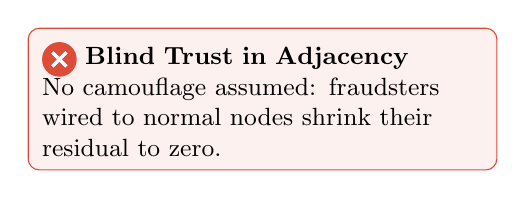
\begin{tikzpicture}
        \node[draw=accent, fill=accent!8, rounded corners, text width=5.6cm, inner sep=5pt, font=\small] (a) {\iconx\ \textbf{Blind Trust in Adjacency}\\ No camouflage assumed: fraudsters wired to normal nodes shrink their residual to zero.};
      \end{tikzpicture}\\[0.25cm]
      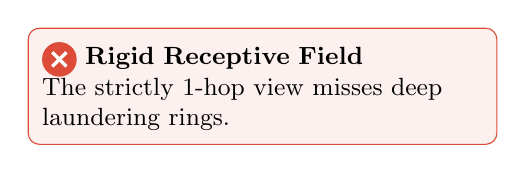
\begin{tikzpicture}
        \node[draw=accent, fill=accent!8, rounded corners, text width=5.6cm, inner sep=5pt, font=\small] (b) {\iconx\ \textbf{Rigid Receptive Field}\\ The strictly 1-hop view misses deep laundering rings.};
      \end{tikzpicture}
    \end{column}
    \begin{column}{0.48\textwidth}
      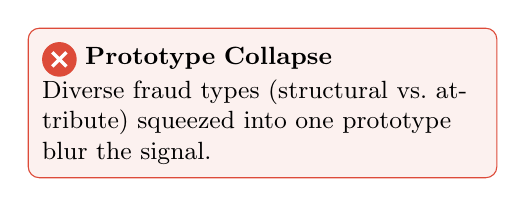
\begin{tikzpicture}
        \node[draw=accent, fill=accent!8, rounded corners, text width=5.6cm, inner sep=5pt, font=\small] (c) {\iconx\ \textbf{Prototype Collapse}\\ Diverse fraud types (structural vs.\ attribute) squeezed into one prototype blur the signal.};
      \end{tikzpicture}\\[0.25cm]
      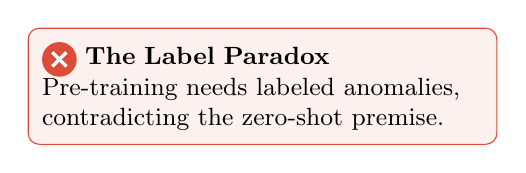
\begin{tikzpicture}
        \node[draw=accent, fill=accent!8, rounded corners, text width=5.6cm, inner sep=5pt, font=\small] (d) {\iconx\ \textbf{The Label Paradox}\\ Pre-training needs labeled anomalies, contradicting the zero-shot premise.};
      \end{tikzpicture}
    \end{column}
    \end{columns}
\end{frame}

% --- SLIDE 4 ---
\begin{frame}{Our Diagnostic Arsenal}
    We built four interventions to patch these structural flaws:
    \vspace{0.2cm}

    \begin{center}
    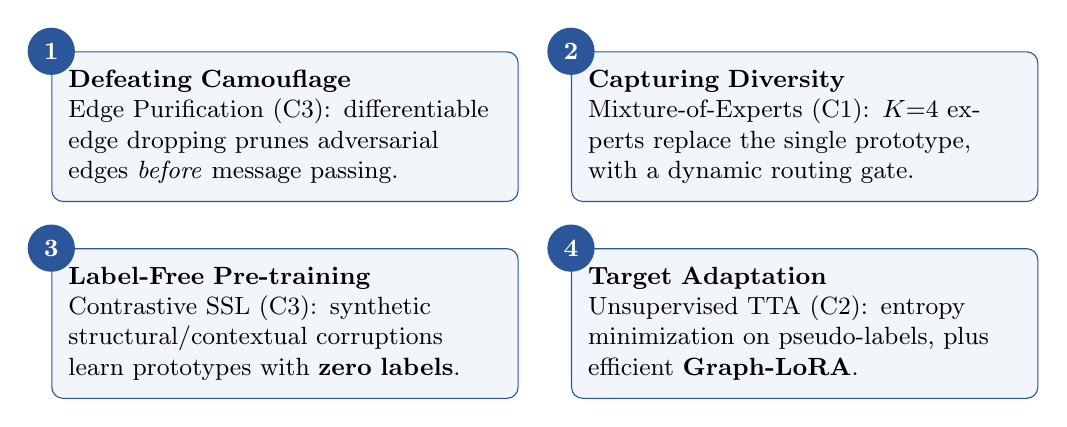
\begin{tikzpicture}[card/.style={draw=primary, fill=primary!6, rounded corners, text width=5.5cm, minimum height=1.9cm, inner sep=6pt, font=\small},
                        num/.style={circle, fill=primary, text=white, font=\bfseries\small, minimum size=0.6cm, inner sep=0pt}]
      \node[card] (c1) at (0,0) {\textbf{Defeating Camouflage}\\Edge Purification (C3): differentiable edge dropping prunes adversarial edges \textit{before} message passing.};
      \node[card] (c2) at (6.6,0) {\textbf{Capturing Diversity}\\Mixture-of-Experts (C1): $K{=}4$ experts replace the single prototype, with a dynamic routing gate.};
      \node[card] (c3) at (0,-2.5) {\textbf{Label-Free Pre-training}\\Contrastive SSL (C3): synthetic structural/contextual corruptions learn prototypes with \textbf{zero labels}.};
      \node[card] (c4) at (6.6,-2.5) {\textbf{Target Adaptation}\\Unsupervised TTA (C2): entropy minimization on pseudo-labels, plus efficient \textbf{Graph-LoRA}.};
      \node[num] at (c1.north west) {1};
      \node[num] at (c2.north west) {2};
      \node[num] at (c3.north west) {3};
      \node[num] at (c4.north west) {4};
    \end{tikzpicture}
    \end{center}
\end{frame}

% --- SLIDE 5 ---
\begin{frame}{Victory 1: Defeating Adversarial Camouflage}
    When anomalies hide behind normal nodes, the baseline is destroyed. Our Edge Purifier survives.

    \vspace{0.3cm}
    \begin{center}
        \fbox{\begin{minipage}{0.8\linewidth}
            \centering
            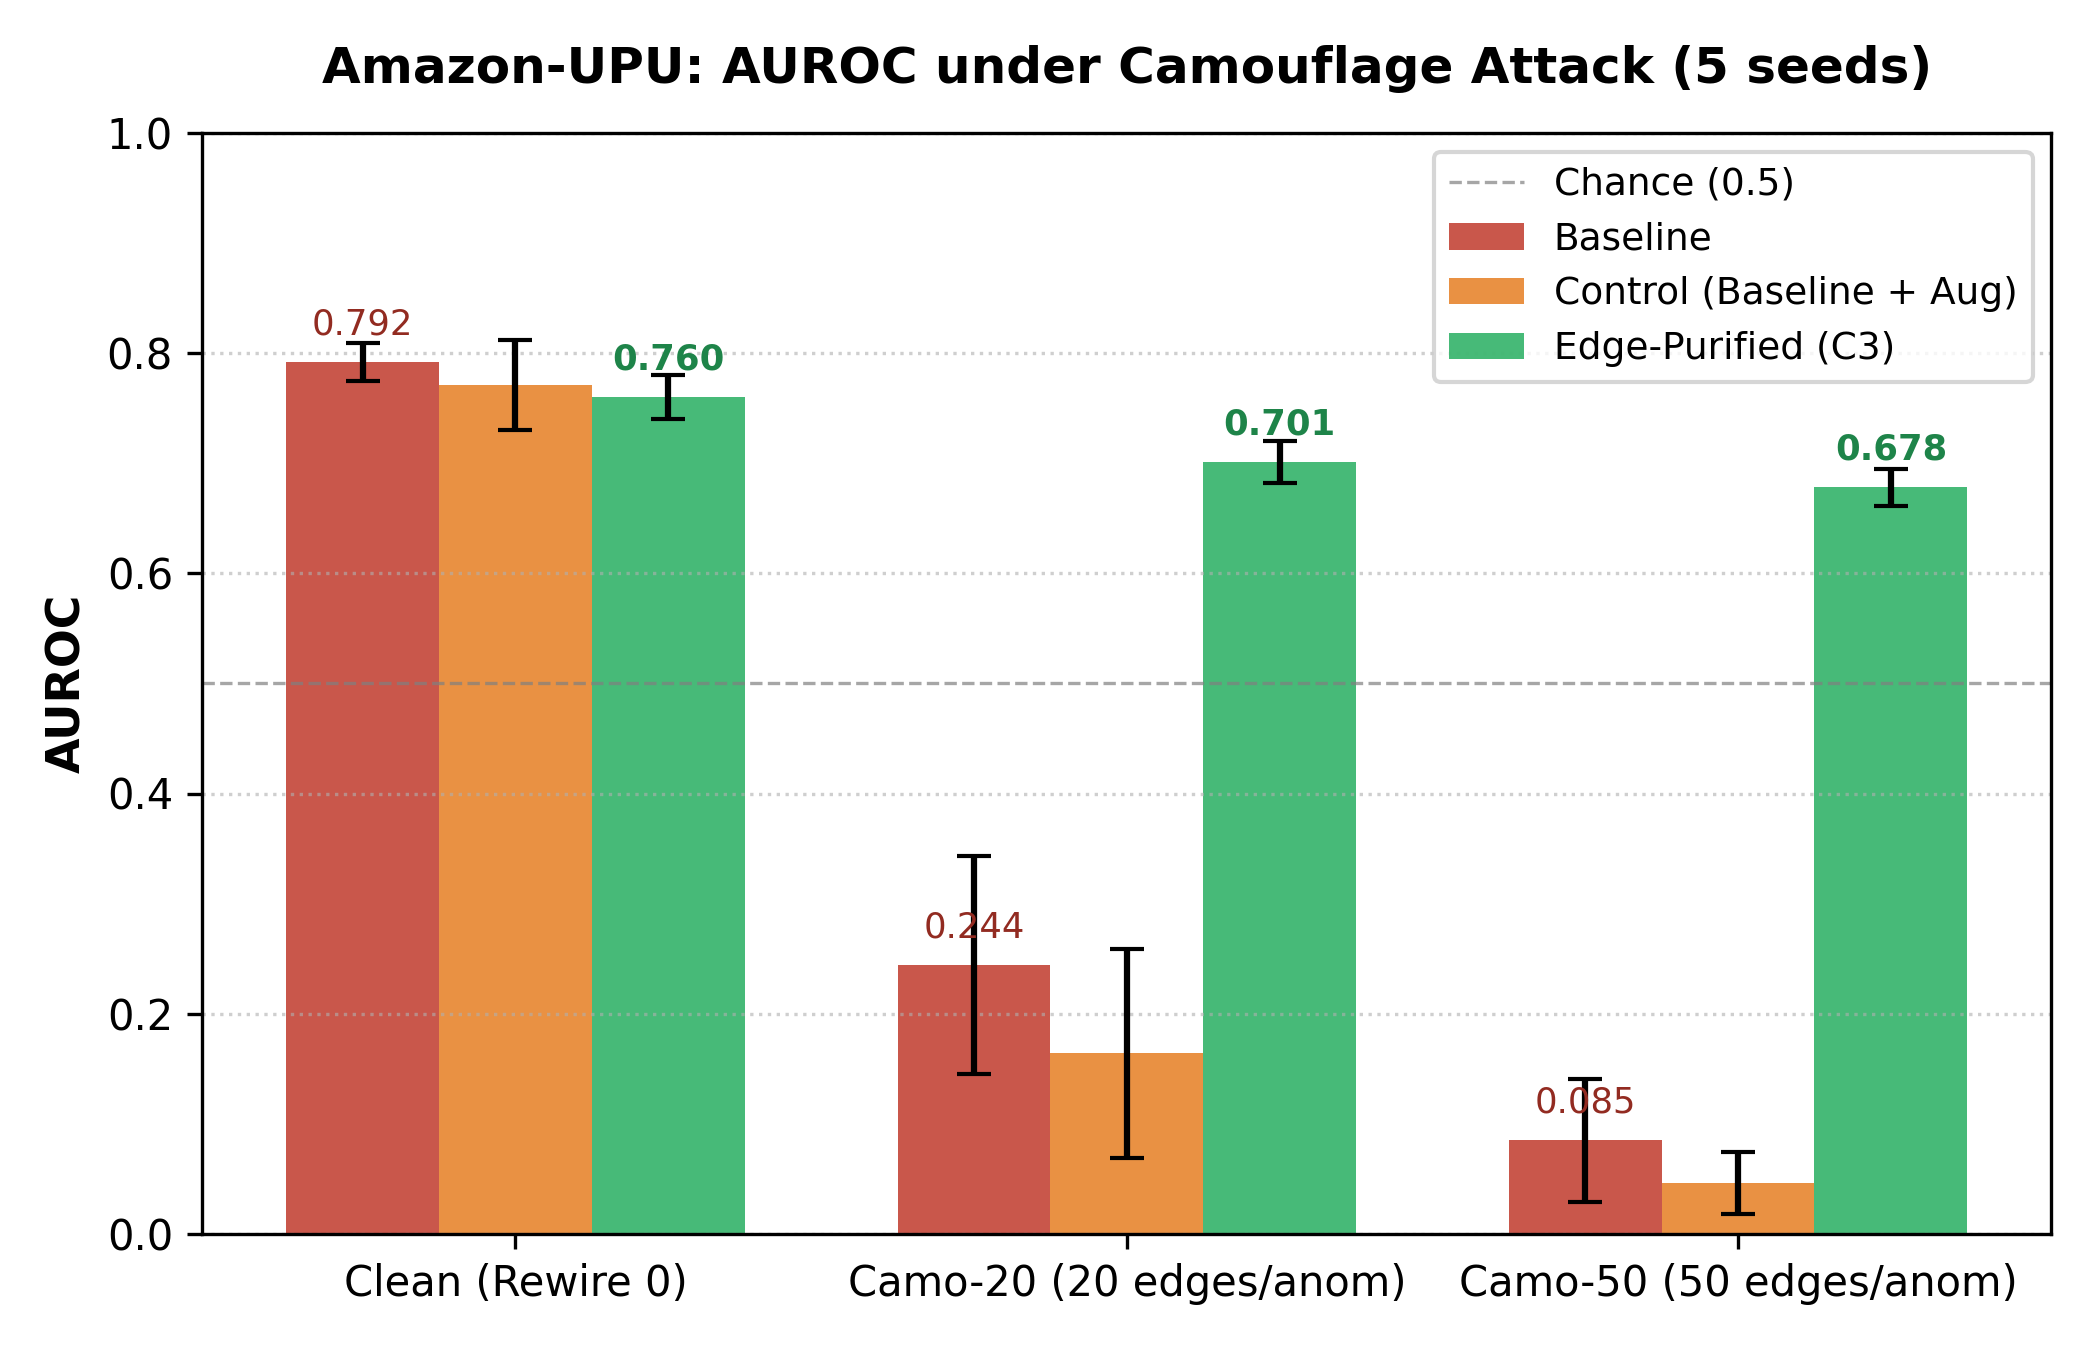
\includegraphics[width=\linewidth,height=4cm,keepaspectratio]{camo_attack_amazon_upu.png}
        \end{minipage}}
    \end{center}

    \vspace{0.3cm}
    \small \textit{Amazon-UPU. Dashed line = chance (0.5). Under a 50-edge attack the baseline ranking inverts (0.085); the purifier drops 99.5\% of injected edges.}
\end{frame}

% --- SLIDE 6 ---
\begin{frame}{Victory 2: Eradicating the Label Dependency}
    Anomaly structure can be learned completely in the dark (zero labels).

    \begin{columns}[c]
        \begin{column}{0.6\textwidth}
            \centering
            \fbox{\begin{minipage}{0.9\linewidth}
                \centering
                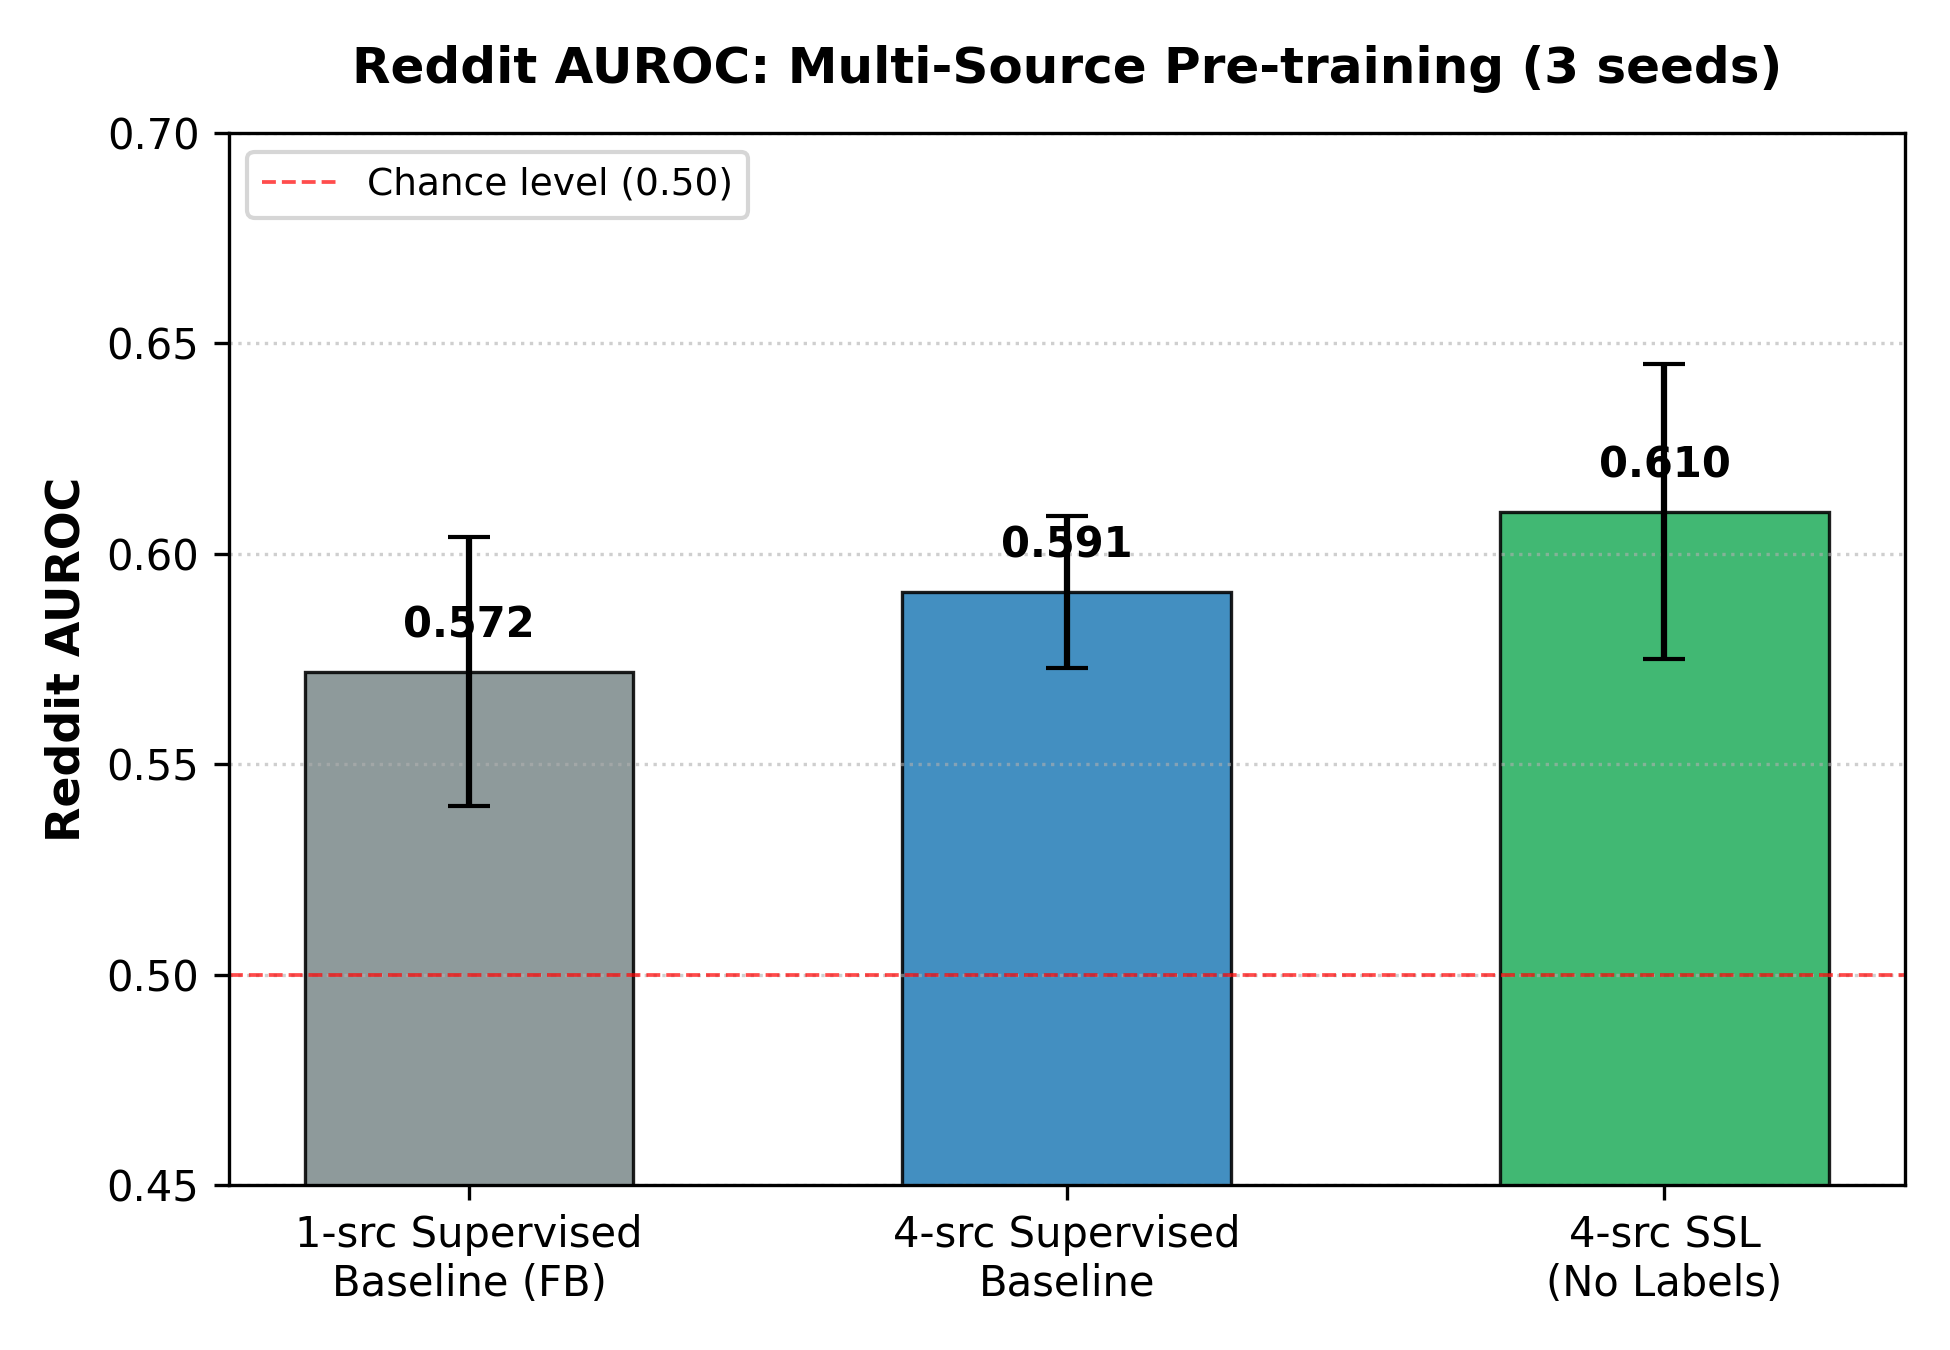
\includegraphics[width=\linewidth,height=3.0cm,keepaspectratio]{ssl_multisource_reddit.png}
            \end{minipage}}
        \end{column}
        \begin{column}{0.36\textwidth}
            \small
            \begin{itemize}
                \item[\iconok] \textbf{0.62 AUROC} on Amazon from synthetic rewiring and feature swaps alone.
                \item[\iconok] Best overall method on Reddit with multi-source pooling.
            \end{itemize}
        \end{column}
    \end{columns}
\end{frame}

% --- SLIDE 7 ---
\begin{frame}{The Structural Transfer Wall}
    Why didn't advanced architectures work everywhere? \textbf{Local topology doesn't always transfer.}

    \vspace{0.2cm}
    \begin{columns}[T]
        \begin{column}{0.48\textwidth}
            \centering
            \fbox{\begin{minipage}{0.9\linewidth}
                \centering
                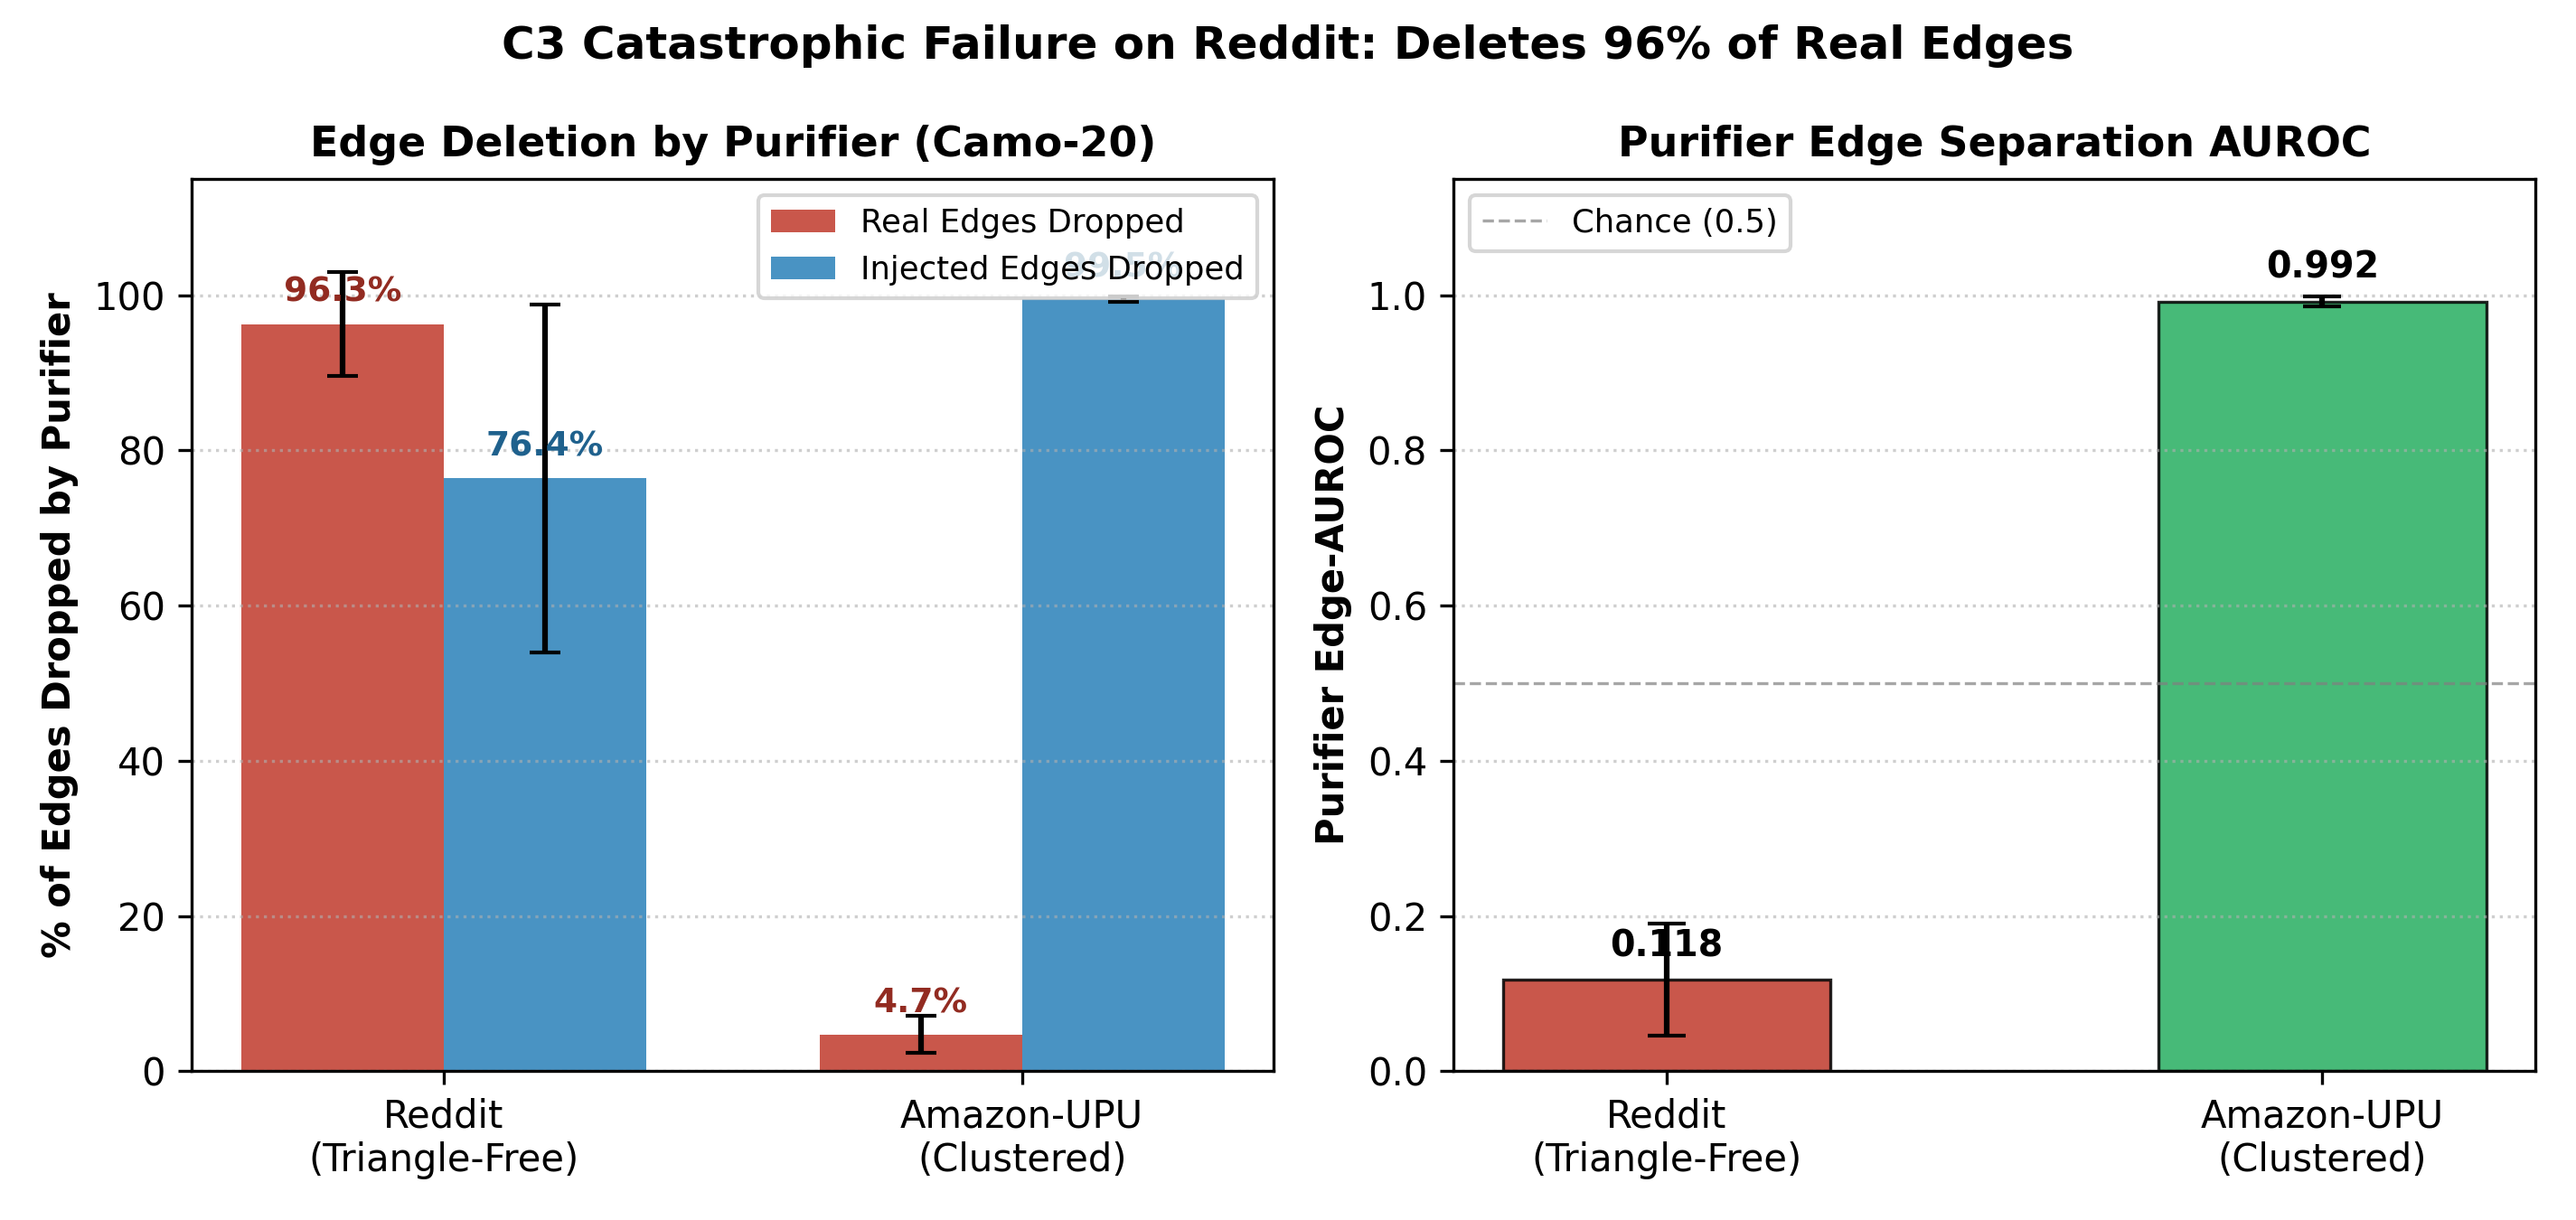
\includegraphics[width=\linewidth,height=3.0cm,keepaspectratio]{purifier_edge_drop_reddit.png}
            \end{minipage}}
            \\[0.2cm]
            {\small \textbf{Purifier failure:} Reddit is triangle-free. The Facebook-trained purifier learned ``no shared neighbors = fake'' and deleted 96\% of real edges.}
        \end{column}

        \begin{column}{0.48\textwidth}
            \centering
            \fbox{\begin{minipage}{0.9\linewidth}
                \centering
                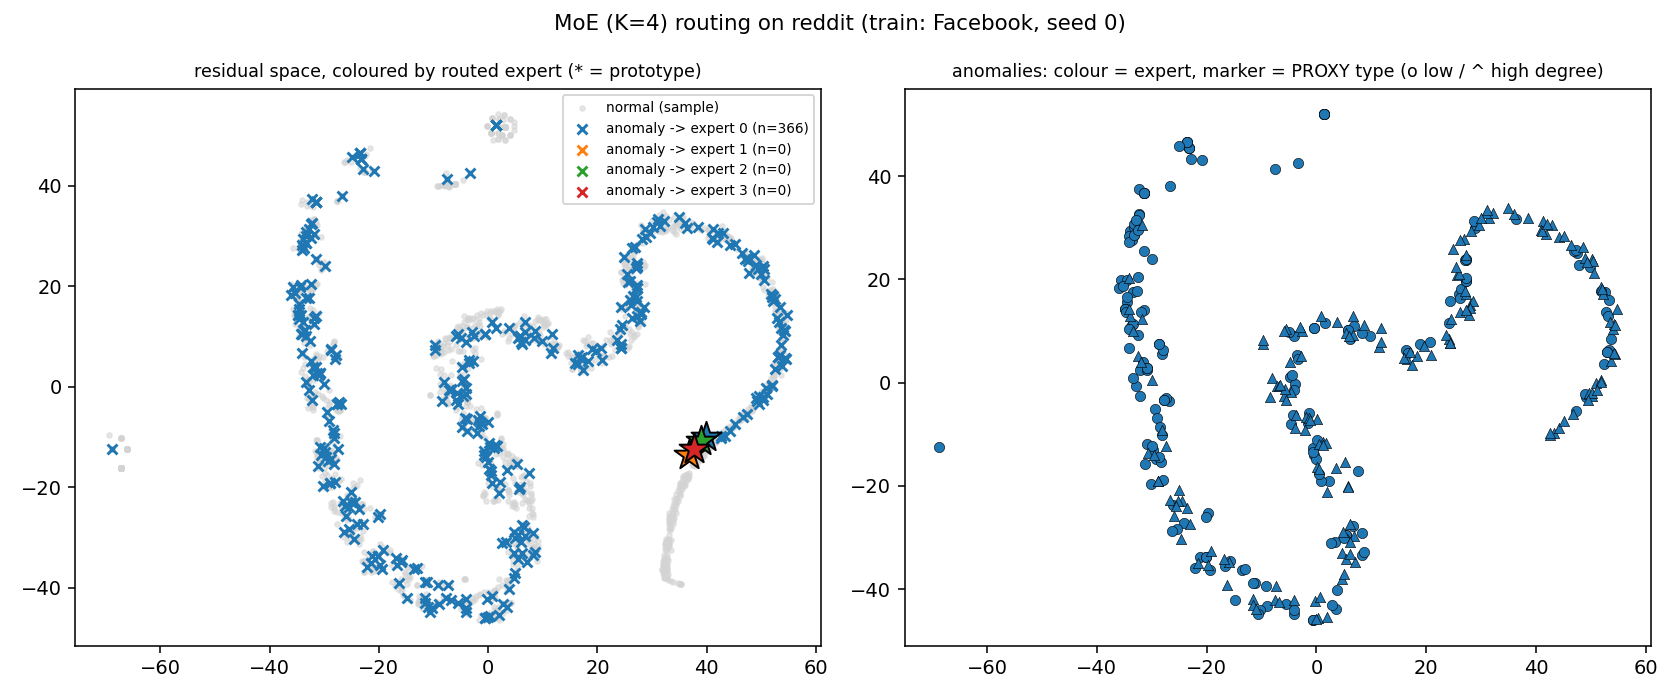
\includegraphics[width=\linewidth,height=3.0cm,keepaspectratio]{moe_tsne_reddit.png}
            \end{minipage}}
            \\[0.2cm]
            {\small \textbf{MoE collapse:} Expert 0 takes 100\% of Reddit anomalies. The router cannot generalize from only $\approx 7$ labeled anomalies.}
        \end{column}
    \end{columns}
\end{frame}

% --- SLIDE 8 ---
\begin{frame}{The Adaptation Paradox}
    Unsupervised Test-Time Adaptation faces a mathematical catch-22.

    \vspace{0.2cm}
    \begin{columns}[T]
        \begin{column}{0.48\textwidth}
            \centering
            \fbox{\begin{minipage}{0.9\linewidth}
                \centering
                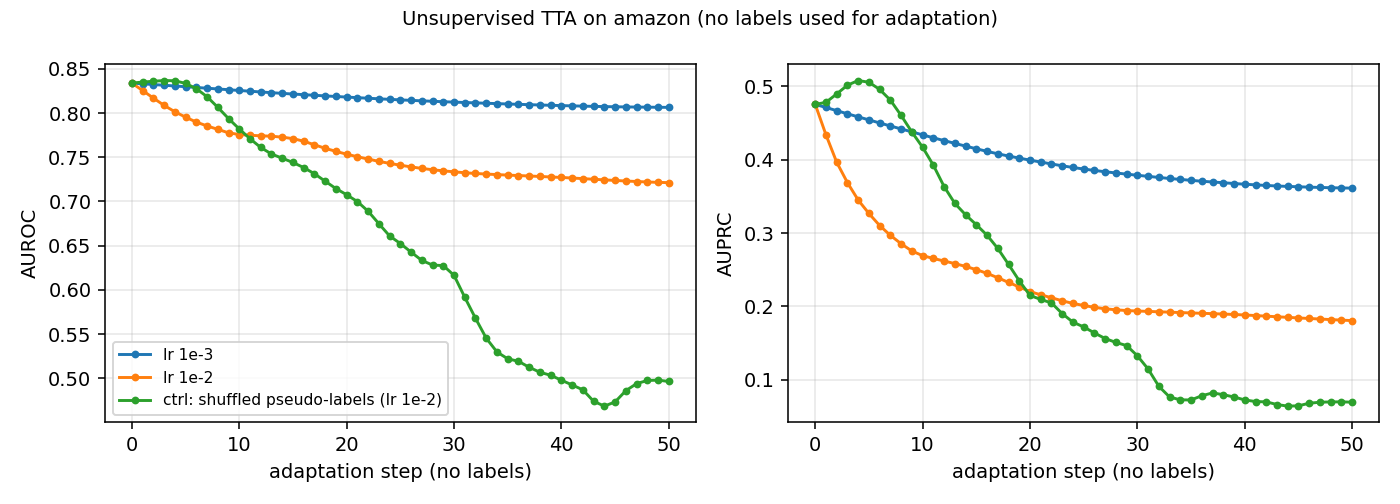
\includegraphics[width=\linewidth,height=3.0cm,keepaspectratio]{tta_curves_amazon.png}
            \end{minipage}}
            \\[0.2cm]
            {\small \textbf{Good graphs (Amazon):} labels are already 75\% accurate, so sharpening an already-good distribution only adds noise.}
        \end{column}

        \begin{column}{0.48\textwidth}
            \centering
            \fbox{\begin{minipage}{0.9\linewidth}
                \centering
                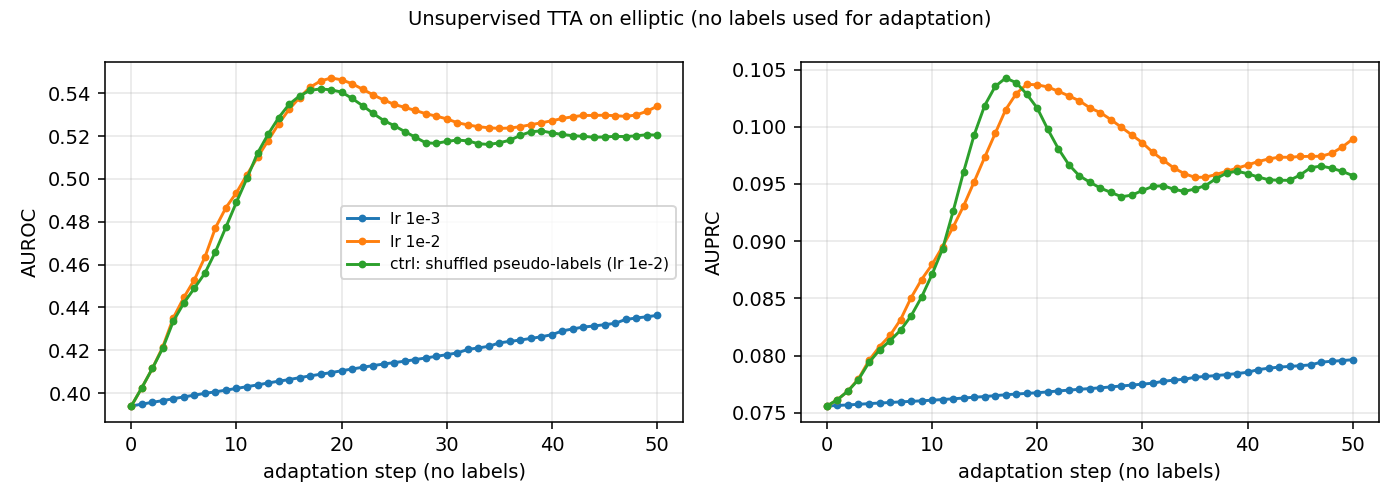
\includegraphics[width=\linewidth,height=3.0cm,keepaspectratio]{tta_curves_elliptic.png}
            \end{minipage}}
            \\[0.2cm]
            {\small \textbf{Bad graphs (Elliptic):} zero-shot ranking is inverted; pseudo-labels are worse than chance. The model learns from pure garbage.}
        \end{column}
    \end{columns}
\end{frame}

% --- SLIDE 9 ---
\begin{frame}{What We Can and Cannot Claim}
    \begin{columns}[T]
        \begin{column}{0.48\textwidth}
            \begin{block}{\iconok\ We CAN Claim}
                \footnotesize
                \begin{itemize}
                    \item \textbf{Camouflage breaks the baseline} (ranking inverts); edge purification fixes it on clustered graphs.
                    \item \textbf{Label-free learning works} via synthetic corruptions.
                    \item \textbf{Graph-LoRA is efficient:} matches full fine-tuning with 2.9\% of the parameters.
                    \item An adaptive PPR gate learns a per-node hop choice.
                \end{itemize}
            \end{block}
        \end{column}

        \begin{column}{0.48\textwidth}
            \begin{block}{\iconx\ We CANNOT Claim}
                \footnotesize
                \begin{itemize}
                    \item \textbf{An average accuracy gain:} no extension beat the baseline on all targets.
                    \item That MoE experts are real anomaly ``types'' (no type labels exist).
                    \item That the purifier works on triangle-free graphs (Reddit) or under heavy random noise.
                    \item Generality beyond the tested targets.
                \end{itemize}
            \end{block}
        \end{column}
    \end{columns}
\end{frame}

% --- SLIDE 10 ---
\begin{frame}{Conclusion \& The Road Ahead}
    \small\sloppy
    \textbf{Verdict:} The bottleneck for Graph Foundation Models is not model capacity, but the limit of single-graph transfer learning and the assumption of structural homogeneity.

    \vspace{0.2cm}
    \begin{center}
    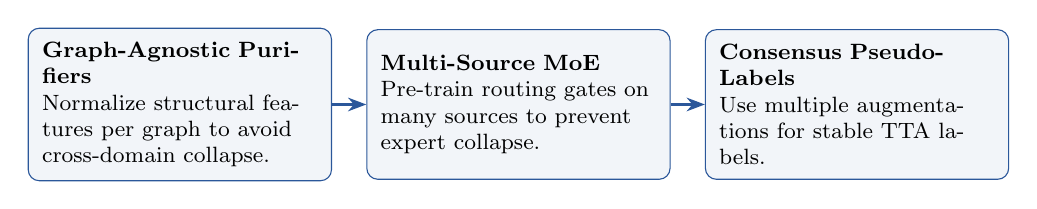
\begin{tikzpicture}[card/.style={draw=primary, fill=primary!6, rounded corners, text width=3.5cm, minimum height=1.9cm, inner sep=5pt, font=\footnotesize, align=left}]
      \node[card] (n1) at (0,0) {\textbf{Graph-Agnostic Purifiers}\\Normalize structural features per graph to avoid cross-domain collapse.};
      \node[card] (n2) at (4.3,0) {\textbf{Multi-Source MoE}\\Pre-train routing gates on many sources to prevent expert collapse.};
      \node[card] (n3) at (8.6,0) {\textbf{Consensus Pseudo-Labels}\\Use multiple augmentations for stable TTA labels.};
      \draw[-{Stealth},thick,primary] (n1)--(n2);
      \draw[-{Stealth},thick,primary] (n2)--(n3);
    \end{tikzpicture}
    \end{center}

    \vspace{0.1cm}
    \begin{center}
    \textbf{Fully reproducible codebase:} \texttt{github.com/SumitKumar-17/AnomalyGFM}\\
    \textit{(Branch: team-contributions, Folder: Anomaly2/)}
    \end{center}
\end{frame}

\end{document}